\documentclass{article}\usepackage[]{graphicx}\usepackage[]{color}
%% maxwidth is the original width if it is less than linewidth
%% otherwise use linewidth (to make sure the graphics do not exceed the margin)
\makeatletter
\def\maxwidth{ %
  \ifdim\Gin@nat@width>\linewidth
    \linewidth
  \else
    \Gin@nat@width
  \fi
}
\makeatother

\definecolor{fgcolor}{rgb}{0.345, 0.345, 0.345}
\newcommand{\hlnum}[1]{\textcolor[rgb]{0.686,0.059,0.569}{#1}}%
\newcommand{\hlstr}[1]{\textcolor[rgb]{0.192,0.494,0.8}{#1}}%
\newcommand{\hlcom}[1]{\textcolor[rgb]{0.678,0.584,0.686}{\textit{#1}}}%
\newcommand{\hlopt}[1]{\textcolor[rgb]{0,0,0}{#1}}%
\newcommand{\hlstd}[1]{\textcolor[rgb]{0.345,0.345,0.345}{#1}}%
\newcommand{\hlkwa}[1]{\textcolor[rgb]{0.161,0.373,0.58}{\textbf{#1}}}%
\newcommand{\hlkwb}[1]{\textcolor[rgb]{0.69,0.353,0.396}{#1}}%
\newcommand{\hlkwc}[1]{\textcolor[rgb]{0.333,0.667,0.333}{#1}}%
\newcommand{\hlkwd}[1]{\textcolor[rgb]{0.737,0.353,0.396}{\textbf{#1}}}%

\usepackage{framed}
\makeatletter
\newenvironment{kframe}{%
 \def\at@end@of@kframe{}%
 \ifinner\ifhmode%
  \def\at@end@of@kframe{\end{minipage}}%
  \begin{minipage}{\columnwidth}%
 \fi\fi%
 \def\FrameCommand##1{\hskip\@totalleftmargin \hskip-\fboxsep
 \colorbox{shadecolor}{##1}\hskip-\fboxsep
     % There is no \\@totalrightmargin, so:
     \hskip-\linewidth \hskip-\@totalleftmargin \hskip\columnwidth}%
 \MakeFramed {\advance\hsize-\width
   \@totalleftmargin\z@ \linewidth\hsize
   \@setminipage}}%
 {\par\unskip\endMakeFramed%
 \at@end@of@kframe}
\makeatother

\definecolor{shadecolor}{rgb}{.97, .97, .97}
\definecolor{messagecolor}{rgb}{0, 0, 0}
\definecolor{warningcolor}{rgb}{1, 0, 1}
\definecolor{errorcolor}{rgb}{1, 0, 0}
\newenvironment{knitrout}{}{} % an empty environment to be redefined in TeX

\usepackage{alltt}

\usepackage[margin = 1in]{geometry}
\usepackage{float, enumitem}
\usepackage{graphicx}
\usepackage{amsmath}

\renewcommand\thesubsection{\thesection (\alph{subsection})}
\IfFileExists{upquote.sty}{\usepackage{upquote}}{}
\begin{document}

\title{ASSIGNMENT 2}
\author{Brandon Lampe \\ STAT 527 \\ Advanced Data Analysis I}
\maketitle

\section{Unseeded vs seeded precipitation:}
The population mean in this problem is of the total rain volume falling from the
cloud base following the airplane seeding run, as measured by radar.  The hypothesis
is that seeding clouds can lead to increased rainfall.

\begin{knitrout}
\definecolor{shadecolor}{rgb}{0.969, 0.969, 0.969}\color{fgcolor}\begin{kframe}
\begin{alltt}
\hlstd{d1} \hlkwb{<-} \hlkwd{read.csv}\hlstd{(}\hlstr{"http://statacumen.com/teach/ADA1/ADA1_HW_02_F14-1.csv"}\hlstd{)}
\hlkwd{library}\hlstd{(ggplot2)}
\hlkwd{library}\hlstd{(grid)}
\hlkwd{library}\hlstd{(gridExtra)}
\hlkwd{source}\hlstd{(}\hlstr{"ADA1_FUNC.R"}\hlstd{)}
\end{alltt}
\end{kframe}
\end{knitrout}

\subsection{Create histogram and boxplot of the unseeded days; then summarize}

\begin{knitrout}
\definecolor{shadecolor}{rgb}{0.969, 0.969, 0.969}\color{fgcolor}\begin{kframe}
\begin{alltt}
\hlcom{# histogram of Unseeded Precip}
\hlstd{Precip.hist} \hlkwb{<-} \hlkwd{ggplot}\hlstd{(d1,} \hlkwd{aes}\hlstd{(}\hlkwc{x} \hlstd{= unseeded))}
\hlstd{Precip.hist} \hlkwb{<-} \hlstd{Precip.hist} \hlopt{+} \hlkwd{geom_histogram}\hlstd{(}\hlkwc{binwidth} \hlstd{=} \hlnum{250}\hlstd{)}
\hlstd{Precip.hist} \hlkwb{<-} \hlstd{Precip.hist} \hlopt{+} \hlkwd{labs}\hlstd{(}\hlkwc{title} \hlstd{=} \hlstr{"Rain Volume [??]"}\hlstd{)}

\hlcom{# boxplot of Unseeded Precip}
\hlstd{Precip.box} \hlkwb{<-} \hlkwd{ggplot}\hlstd{(d1,} \hlkwd{aes}\hlstd{(}\hlkwc{x} \hlstd{=} \hlstr{"Volume"}\hlstd{,} \hlkwc{y} \hlstd{= unseeded))} \hlcom{# boxplot of Precip}
\hlstd{Precip.box} \hlkwb{<-} \hlstd{Precip.box} \hlopt{+} \hlkwd{geom_boxplot}\hlstd{()}
\hlstd{Precip.box} \hlkwb{<-} \hlstd{Precip.box} \hlopt{+} \hlkwd{coord_flip}\hlstd{()}
\hlstd{Precip.box} \hlkwb{<-} \hlstd{Precip.box} \hlopt{+} \hlkwd{labs}\hlstd{(}\hlkwc{title} \hlstd{=} \hlstr{"Rain Volume [??]"}\hlstd{)}

\hlcom{# plot histogram and boxplot}
\hlkwd{grid.arrange}\hlstd{(Precip.hist, Precip.box,} \hlkwc{ncol} \hlstd{=} \hlnum{2}\hlstd{)}
\end{alltt}
\end{kframe}
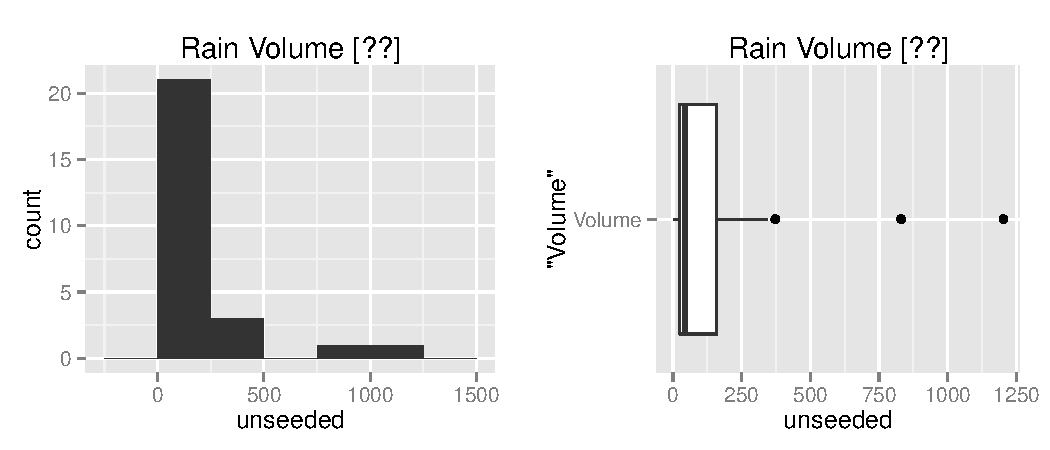
\includegraphics[width=\maxwidth]{figure/1a_} 

\end{knitrout}


\begin{knitrout}
\definecolor{shadecolor}{rgb}{0.969, 0.969, 0.969}\color{fgcolor}\begin{kframe}
\begin{alltt}
\hlkwd{mean}\hlstd{(d1}\hlopt{$}\hlstd{unseeded)}
\end{alltt}
\begin{verbatim}
## [1] 164.6
\end{verbatim}
\begin{alltt}
\hlkwd{median}\hlstd{(d1}\hlopt{$}\hlstd{unseeded)}
\end{alltt}
\begin{verbatim}
## [1] 44.2
\end{verbatim}
\begin{alltt}
\hlkwd{sd}\hlstd{(d1}\hlopt{$}\hlstd{unseeded)}
\end{alltt}
\begin{verbatim}
## [1] 278.4
\end{verbatim}
\begin{alltt}
\hlkwd{diff}\hlstd{(}\hlkwd{fivenum}\hlstd{(d1}\hlopt{$}\hlstd{unseeded)[}\hlkwd{c}\hlstd{(}\hlnum{2}\hlstd{,}\hlnum{4}\hlstd{)])} \hlcom{#IQR}
\end{alltt}
\begin{verbatim}
## [1] 138.6
\end{verbatim}
\begin{alltt}
\hlkwd{fivenum}\hlstd{(d1}\hlopt{$}\hlstd{unseeded)}
\end{alltt}
\begin{verbatim}
## [1]    1.0   24.4   44.2  163.0 1202.6
\end{verbatim}
\end{kframe}
\end{knitrout}

The distribution is unimodal, unsymmetric, skewed right, not normal, and has three outliers.
$\bar{Y} - M = 164.6 - 44.2 = 120.4$, which is very large and consistent with
observed skewness.
No units were provided with the data; therefore, a quantitative analysis is difficult.
The data represents volume of rain from clouds that were not seeded; therefore,
this data essentially provides a measure of the volume of rain from a cumulus
cloud, which often produce little to no precipitation.

\subsection{Obtain a 95\% confidence interval}

\begin{knitrout}
\definecolor{shadecolor}{rgb}{0.969, 0.969, 0.969}\color{fgcolor}\begin{kframe}
\begin{alltt}
\hlcom{# Manually calculate confidence interval}
\hlstd{us.sd}     \hlkwb{<-} \hlkwd{sd}\hlstd{(d1}\hlopt{$}\hlstd{unseeded)}        \hlcom{# standard deviation unseeded}
\hlstd{us.ct}     \hlkwb{<-} \hlkwd{length}\hlstd{(d1}\hlopt{$}\hlstd{unseeded)}    \hlcom{# count of unseeded}
\hlstd{us.SEM}    \hlkwb{<-} \hlstd{us.sd}\hlopt{/}\hlkwd{sqrt}\hlstd{(us.ct} \hlopt{-} \hlnum{1}\hlstd{)}  \hlcom{# standard error of the mean}
\hlstd{us.M}      \hlkwb{<-} \hlkwd{mean}\hlstd{(d1}\hlopt{$}\hlstd{unseeded)}      \hlcom{# mean}
\hlstd{us.alpha}  \hlkwb{<-} \hlnum{0.05}                   \hlcom{# alpha value, for CI = 95%}

\hlkwd{abs}\hlstd{(}\hlkwd{qt}\hlstd{(us.alpha}\hlopt{/}\hlnum{2}\hlstd{,} \hlkwc{df} \hlstd{= us.ct} \hlopt{-} \hlnum{1}\hlstd{))} \hlcom{# two sided t_crit}
\end{alltt}
\begin{verbatim}
## [1] 2.06
\end{verbatim}
\begin{alltt}
\hlstd{us.UL}     \hlkwb{<-} \hlstd{us.M} \hlopt{+} \hlstd{us.tcrit}\hlopt{*}\hlstd{us.SEM} \hlcom{# upper limit of 95% CI}
\end{alltt}


{\ttfamily\noindent\bfseries\color{errorcolor}{\#\# Error: object 'us.tcrit' not found}}\begin{alltt}
\hlstd{us.LL}     \hlkwb{<-} \hlstd{us.M} \hlopt{-} \hlstd{us.tcrit}\hlopt{*}\hlstd{us.SEM} \hlcom{# lower limit of 95% CI}
\end{alltt}


{\ttfamily\noindent\bfseries\color{errorcolor}{\#\# Error: object 'us.tcrit' not found}}\begin{alltt}
\hlcom{# Use function to calculate confidence interval}
\hlkwd{t.test}\hlstd{(d1}\hlopt{$}\hlstd{unseeded,} \hlkwc{mu} \hlstd{= us.M)} \hlcom{# Student's t-test function}
\end{alltt}
\begin{verbatim}
## 
## 	One Sample t-test
## 
## data:  d1$unseeded
## t = 0, df = 25, p-value = 1
## alternative hypothesis: true mean is not equal to 164.6
## 95 percent confidence interval:
##   52.13 277.05
## sample estimates:
## mean of x 
##     164.6
\end{verbatim}
\begin{alltt}
\hlcom{#peform bootstrap sampling to determine if the distribution is normal}
\hlkwd{bs.one.samp.dist}\hlstd{(d1}\hlopt{$}\hlstd{unseeded)}
\end{alltt}
\end{kframe}
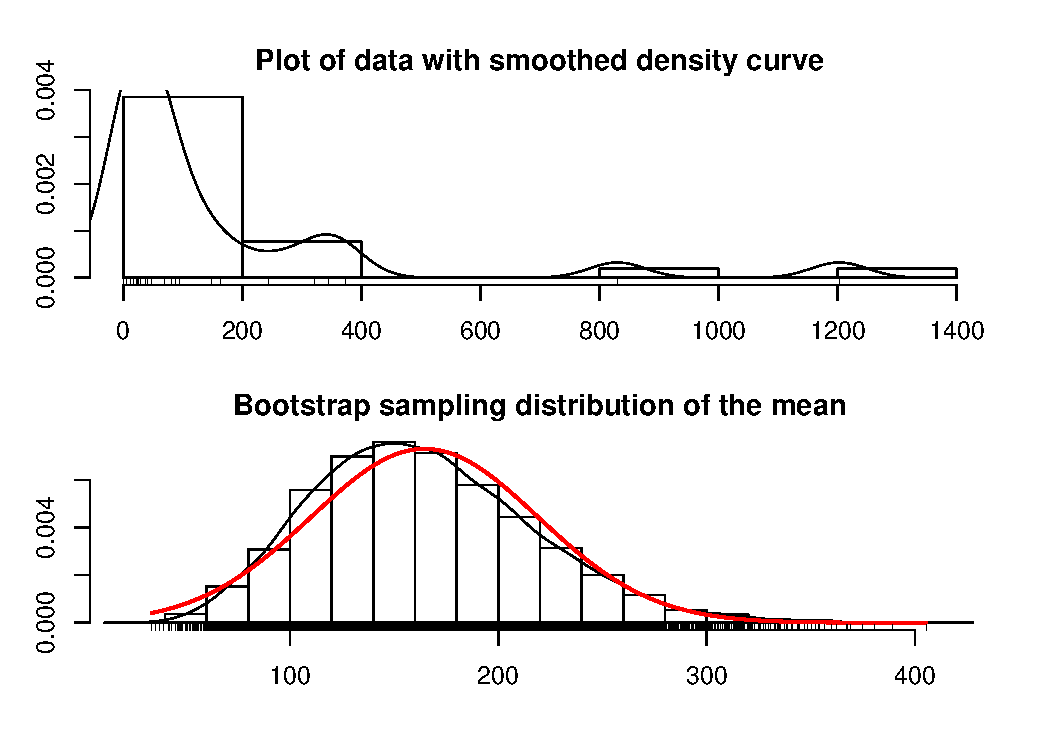
\includegraphics[width=\maxwidth]{figure/1b} 

\end{knitrout}

The 95\% Confidence Interval = 164.6 $\pm$ 112.5.
Therefore, with 95\% confidence the mean of unseeded rainfall volume will be betwee
52 and 278.\\

The assumptions for the t-test and the corresponding confidence interval are:
\begin{itemize}
  \item Data are a random sample from the population
  \item Population frequency curve is normal
\end{itemize}

The population of cumulus clouds were randomly seeded by the meachanism.
However, using the bootstrop method, the data are skewed right and
not normally distributed, which is contrary to the underlying assumpionts
used to calculated the confidence interval.  The normality assumption was not met.

\subsection{Transform the data by taking the log() of each value}

\begin{knitrout}
\definecolor{shadecolor}{rgb}{0.969, 0.969, 0.969}\color{fgcolor}\begin{kframe}
\begin{alltt}
\hlstd{logd1} \hlkwb{<-} \hlkwd{log}\hlstd{(d1)} \hlcom{# natural log of data}

\hlstd{logd1.hist} \hlkwb{<-} \hlkwd{ggplot}\hlstd{(logd1,} \hlkwd{aes}\hlstd{(}\hlkwc{x} \hlstd{= unseeded))}
\hlstd{logd1.hist} \hlkwb{<-} \hlstd{logd1.hist} \hlopt{+} \hlkwd{geom_histogram}\hlstd{(}\hlkwc{binwidth} \hlstd{=} \hlnum{1}\hlstd{)}
\hlstd{logd1.hist} \hlkwb{<-} \hlstd{logd1.hist} \hlopt{+} \hlkwd{labs}\hlstd{(}\hlkwc{title} \hlstd{=} \hlstr{"Rain Volume [??]"}\hlstd{)}

\hlcom{# boxplot of Unseeded logd1}
\hlstd{logd1.box} \hlkwb{<-} \hlkwd{ggplot}\hlstd{(logd1,} \hlkwd{aes}\hlstd{(}\hlkwc{x} \hlstd{=} \hlstr{"Volume"}\hlstd{,} \hlkwc{y} \hlstd{= unseeded))} \hlcom{# boxplot of logd1}
\hlstd{logd1.box} \hlkwb{<-} \hlstd{logd1.box} \hlopt{+} \hlkwd{geom_boxplot}\hlstd{()}
\hlstd{logd1.box} \hlkwb{<-} \hlstd{logd1.box} \hlopt{+} \hlkwd{coord_flip}\hlstd{()}
\hlstd{logd1.box} \hlkwb{<-} \hlstd{logd1.box} \hlopt{+} \hlkwd{labs}\hlstd{(}\hlkwc{title} \hlstd{=} \hlstr{"Rain Volume [??]"}\hlstd{)}

\hlcom{# plot histogram and boxplot}
\hlkwd{grid.arrange}\hlstd{(logd1.hist, logd1.box,} \hlkwc{ncol} \hlstd{=} \hlnum{1}\hlstd{)}
\end{alltt}
\end{kframe}
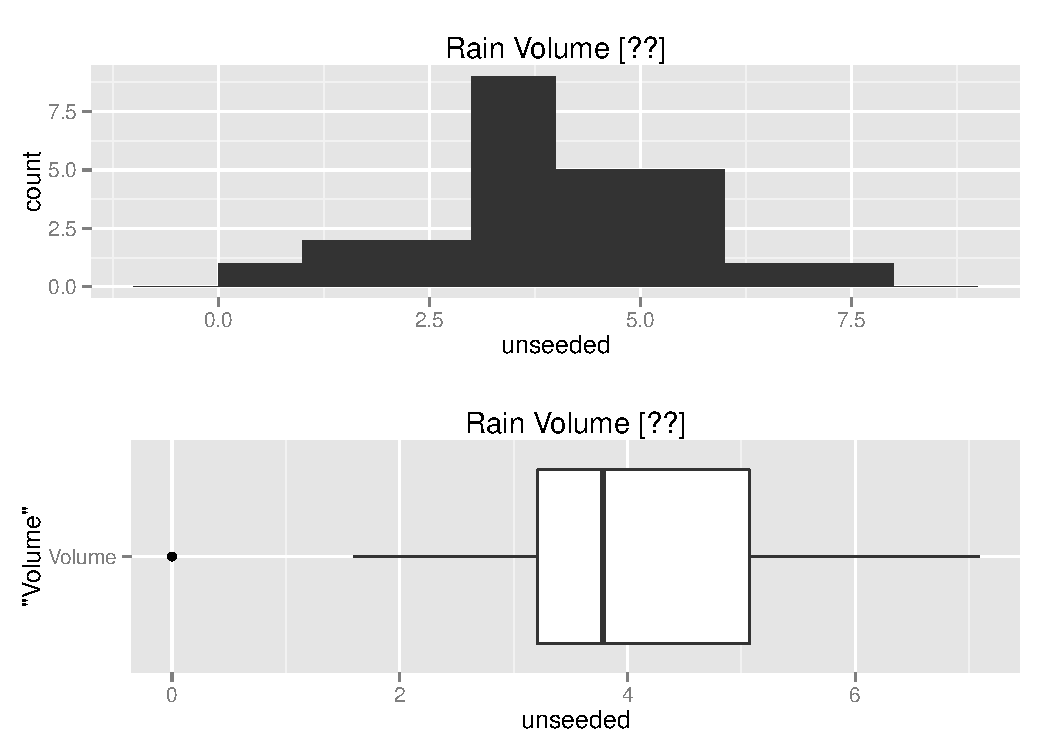
\includegraphics[width=\maxwidth]{figure/1c} 
\begin{kframe}\begin{alltt}
\hlkwd{mean}\hlstd{(logd1}\hlopt{$}\hlstd{unseeded)}
\end{alltt}
\begin{verbatim}
## [1] 3.99
\end{verbatim}
\begin{alltt}
\hlkwd{median}\hlstd{(logd1}\hlopt{$}\hlstd{unseeded)}
\end{alltt}
\begin{verbatim}
## [1] 3.786
\end{verbatim}
\begin{alltt}
\hlkwd{sd}\hlstd{(logd1}\hlopt{$}\hlstd{unseeded)}
\end{alltt}
\begin{verbatim}
## [1] 1.642
\end{verbatim}
\begin{alltt}
\hlkwd{diff}\hlstd{(}\hlkwd{fivenum}\hlstd{(logd1}\hlopt{$}\hlstd{unseeded)[}\hlkwd{c}\hlstd{(}\hlnum{2}\hlstd{,}\hlnum{4}\hlstd{)])} \hlcom{#IQR}
\end{alltt}
\begin{verbatim}
## [1] 1.899
\end{verbatim}
\begin{alltt}
\hlkwd{fivenum}\hlstd{(logd1}\hlopt{$}\hlstd{unseeded)}
\end{alltt}
\begin{verbatim}
## [1] 0.000 3.195 3.786 5.094 7.092
\end{verbatim}
\end{kframe}
\end{knitrout}

The transformed distribution is unimodal, symmetric, close to normal, with one outlier.
$\bar{Y} - M = 3.99 - 3.79 = 0.2$ is fairly small relative to the variability,
which is consistent with the observed symmetry.

\subsection{Obtain a 95\% confidence interval for the mean log()}
\begin{knitrout}
\definecolor{shadecolor}{rgb}{0.969, 0.969, 0.969}\color{fgcolor}\begin{kframe}
\begin{alltt}
\hlcom{# Use function to calculate confidence interval}
\hlkwd{abs}\hlstd{(}\hlkwd{qt}\hlstd{(}\hlnum{.025}\hlstd{,} \hlkwc{df} \hlstd{= us.ct} \hlopt{-} \hlnum{1}\hlstd{))} \hlcom{# two sided t_crit}
\end{alltt}
\begin{verbatim}
## [1] 2.06
\end{verbatim}
\begin{alltt}
\hlkwd{t.test}\hlstd{(logd1}\hlopt{$}\hlstd{unseeded)} \hlcom{# Student's t-test function}
\end{alltt}
\begin{verbatim}
## 
## 	One Sample t-test
## 
## data:  logd1$unseeded
## t = 12.39, df = 25, p-value = 3.59e-12
## alternative hypothesis: true mean is not equal to 0
## 95 percent confidence interval:
##  3.327 4.654
## sample estimates:
## mean of x 
##      3.99
\end{verbatim}
\begin{alltt}
\hlcom{#peform bootstrap sampling to determine if the distribution is normal}
\hlkwd{bs.one.samp.dist}\hlstd{(logd1}\hlopt{$}\hlstd{unseeded)}
\end{alltt}
\end{kframe}
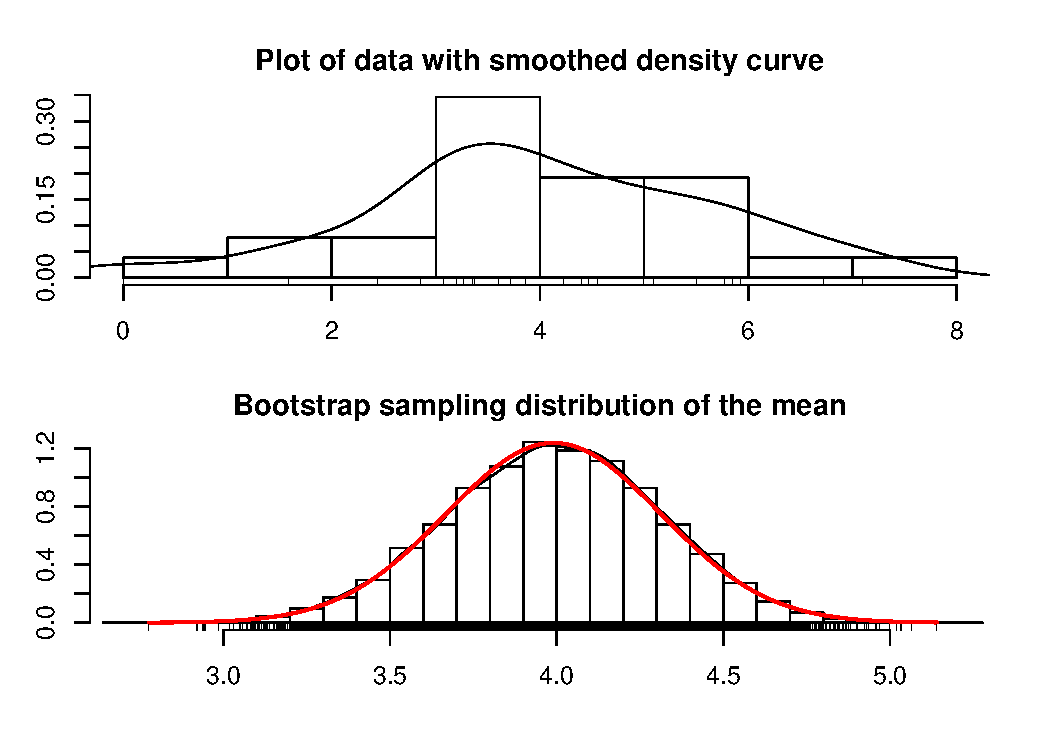
\includegraphics[width=\maxwidth]{figure/1_d} 

\end{knitrout}

The 95\% confidence interval of the log of the mean unseeded precipitation data
is from 3.4 to 4.7.\\
Yes, the assumptions for this method appear to be appropriate because the data
were randomly sampled and the Bootstrap sampling of the data are normally distributed.

\section{TCL}
\begin{knitrout}
\definecolor{shadecolor}{rgb}{0.969, 0.969, 0.969}\color{fgcolor}\begin{kframe}
\begin{alltt}
\hlstd{d2} \hlkwb{<-} \hlkwd{read.csv}\hlstd{(}\hlstr{"http://statacumen.com/teach/ADA1/ADA1_HW_02_F14-2.csv"}\hlstd{)}
\end{alltt}
\end{kframe}
\end{knitrout}


\subsection{}
\begin{enumerate}[label=(\Alph*)]
  \item \textbf{define the population parameter:} The population parameter is the mean TCL
    of young adult males on the Kaiser plan.  $\mu = $ mean TCL of young adult
    males on the Kaiser plan.

  \item \textbf{state the hypothesis:}  The hypothesis is that the TCL of young adult males
  on the Kaiser plan is equal to the mean TCL of all adult males in the United
  States, which is 210.  $H_0: \mu = 210$ against $H_A: \mu \neq 210$.

  \item \textbf{state assumptions and how they will be assessed:}  The assumptions for
  this analysis are that the data are normally distributed and they data were
  randomly sampled.  Normality will be assessed using the bootstrap method where
  10,000 proxy samples are randomly drawn from the full sample.  The mean of each
  proxy sample is then calculated and plotted against a normal distribution curve.
  If the distribution of the bootstrap (proxy) samples appears normal, then the
  normality assumption is valid.  No information is provided regarding the randomness
  of the sample population; therefore, I will assume it was randomly obtained.

  \item \textbf{evaluate assumptions based on graphical summaries:}
\begin{knitrout}
\definecolor{shadecolor}{rgb}{0.969, 0.969, 0.969}\color{fgcolor}\begin{kframe}
\begin{alltt}
\hlkwd{bs.one.samp.dist}\hlstd{(d2}\hlopt{$}\hlstd{TCL)}      \hlcom{# plot histogram and frequency density curve}
\end{alltt}
\end{kframe}
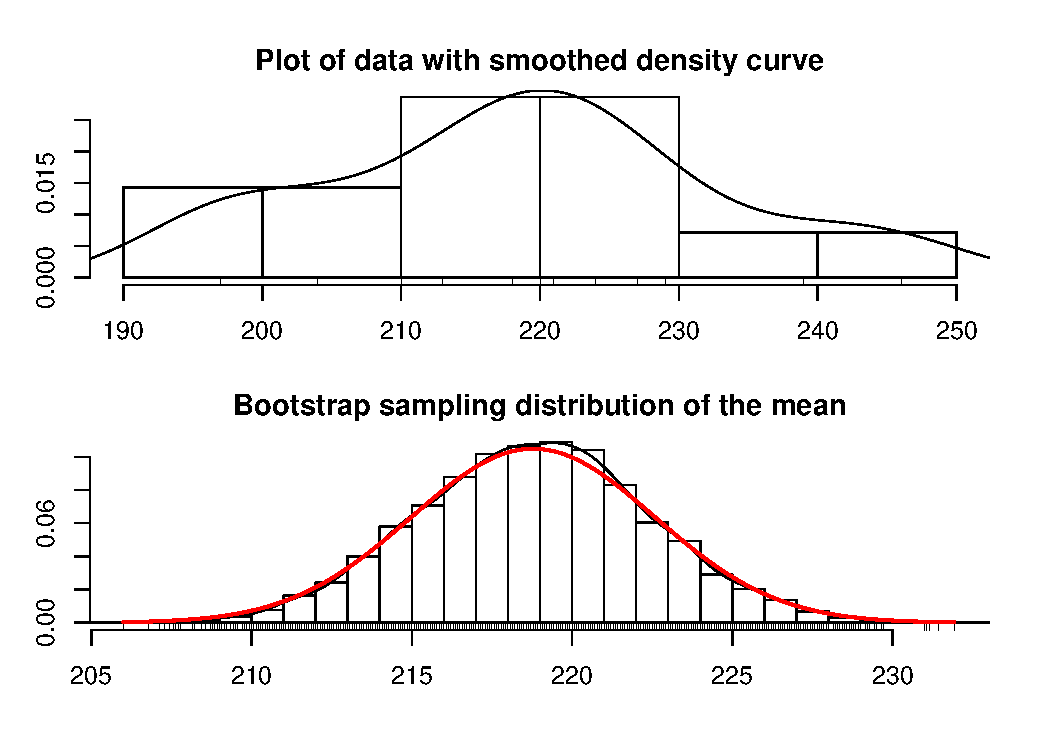
\includegraphics[width=\maxwidth]{figure/2ad} 

\end{knitrout}

\begin{knitrout}
\definecolor{shadecolor}{rgb}{0.969, 0.969, 0.969}\color{fgcolor}\begin{kframe}
\begin{alltt}
\hlcom{# plot box plot}
\hlstd{d2.box} \hlkwb{<-} \hlkwd{ggplot}\hlstd{(d2,} \hlkwd{aes}\hlstd{(}\hlkwc{x} \hlstd{=} \hlstr{"TCL"}\hlstd{,} \hlkwc{y} \hlstd{= TCL))} \hlcom{# boxplot of d2}
\hlstd{d2.box} \hlkwb{<-} \hlstd{d2.box} \hlopt{+} \hlkwd{geom_boxplot}\hlstd{()}
\hlstd{d2.box} \hlkwb{<-} \hlstd{d2.box} \hlopt{+} \hlkwd{coord_flip}\hlstd{()}
\hlstd{d2.box} \hlkwb{<-} \hlstd{d2.box} \hlopt{+} \hlkwd{stat_summary}\hlstd{(}\hlkwc{fun.y} \hlstd{= mean,} \hlkwc{geom} \hlstd{=} \hlstr{"point"}\hlstd{,} \hlkwc{shape} \hlstd{=} \hlnum{3}\hlstd{,} \hlkwc{size} \hlstd{=} \hlnum{2}\hlstd{)}
\hlstd{d2.box} \hlkwb{<-} \hlstd{d2.box} \hlopt{+} \hlkwd{labs}\hlstd{(}\hlkwc{title} \hlstd{=} \hlstr{"TCLs for Young Adult Males on the Kaiser Health Plan in California"}\hlstd{)}
\hlstd{d2.box}
\end{alltt}
\end{kframe}
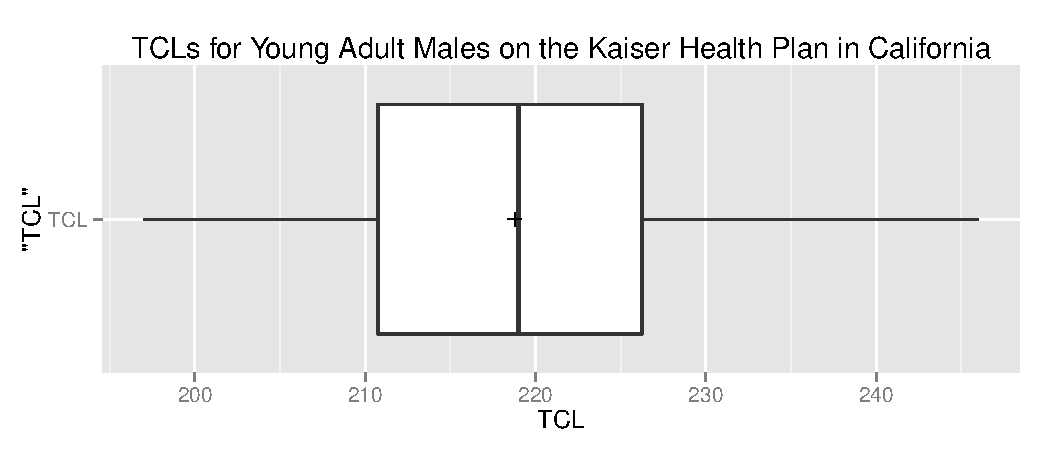
\includegraphics[width=\maxwidth]{figure/2ad2} 

\end{knitrout}

  Based on the histogram of the sample data, the data are unimodal, symmetric,
  and nearly normal.  Based on the bootstrap distribution, the sample data are
  normally distributed.  The boxplot of sample data shows that no outliers exist,
  the tails are approximately equal, and the mean is very near the meadian.


  \item \textbf{discuss the test and the decision:}

\begin{knitrout}
\definecolor{shadecolor}{rgb}{0.969, 0.969, 0.969}\color{fgcolor}\begin{kframe}
\begin{alltt}
\hlstd{ybar} \hlkwb{<-} \hlkwd{mean}\hlstd{(d2}\hlopt{$}\hlstd{TCL)}\hlcom{# mean of sample}
\hlstd{s} \hlkwb{<-} \hlkwd{sd}\hlstd{(d2}\hlopt{$}\hlstd{TCL)}     \hlcom{# standard deviation}
\hlstd{n} \hlkwb{<-} \hlkwd{length}\hlstd{(d2}\hlopt{$}\hlstd{TCL)} \hlcom{# observations in sampe}
\hlstd{SEM} \hlkwb{<-} \hlstd{s}\hlopt{/}\hlkwd{sqrt}\hlstd{(n)}    \hlcom{# standard error of the mean}
\hlstd{df} \hlkwb{<-} \hlstd{n} \hlopt{-} \hlnum{1}         \hlcom{# degrees of freedom}
\hlstd{tcrit} \hlkwb{<-}\hlkwd{qt}\hlstd{(}\hlnum{.025}\hlstd{, df)}\hlcom{# t_crit}
\hlstd{M} \hlkwb{<-} \hlkwd{median}\hlstd{(d2}\hlopt{$}\hlstd{TCL)}\hlcom{# median}

\hlnum{210} \hlopt{-} \hlstd{tcrit}\hlopt{*}\hlstd{SEM}
\end{alltt}
\begin{verbatim}
## [1] 218.2
\end{verbatim}
\begin{alltt}
\hlnum{210} \hlopt{+} \hlstd{tcrit} \hlopt{*} \hlstd{SEM}
\end{alltt}
\begin{verbatim}
## [1] 201.8
\end{verbatim}
\begin{alltt}
\hlstd{d2.t} \hlkwb{<-} \hlkwd{t.test}\hlstd{(d2,} \hlkwc{mu} \hlstd{=} \hlnum{210}\hlstd{)}  \hlcom{# t-test summary}
\hlstd{d2.t}
\end{alltt}
\begin{verbatim}
## 
## 	One Sample t-test
## 
## data:  d2
## t = 2.309, df = 13, p-value = 0.038
## alternative hypothesis: true mean is not equal to 210
## 95 percent confidence interval:
##  210.6 227.0
## sample estimates:
## mean of x 
##     218.8
\end{verbatim}
\end{kframe}
\end{knitrout}

The sample summaries are $n = 14, \bar{Y} = 218.8, s = 14.2 \text{ and }
SE_{\bar{Y}} = 3.80$.  $\bar{Y} - M = 218.8 - 219 = 0.02$ is very small
relative to the variability, which is consistent with the observed symmetry.

I reject $H_0$ in favor of $H_A$.  This test was performed at a 5\% level
(i.e. $\alpha = 0.05$), and the p-value (0.038) is $\le \alpha$ and
accordingly $t_s (2.309) \ge t_{crit}(2.16)$.  The data suggest that
$\mu \neq 210$.

\end{enumerate}

\subsection{}
\begin{knitrout}
\definecolor{shadecolor}{rgb}{0.969, 0.969, 0.969}\color{fgcolor}\begin{kframe}
\begin{alltt}
\hlkwd{t.test}\hlstd{(d2,} \hlkwc{mu} \hlstd{=} \hlnum{210}\hlstd{)}
\end{alltt}
\begin{verbatim}
## 
## 	One Sample t-test
## 
## data:  d2
## t = 2.309, df = 13, p-value = 0.038
## alternative hypothesis: true mean is not equal to 210
## 95 percent confidence interval:
##  210.6 227.0
## sample estimates:
## mean of x 
##     218.8
\end{verbatim}
\begin{alltt}
\hlkwd{IQR}\hlstd{(d2}\hlopt{$}\hlstd{TCL)}
\end{alltt}
\begin{verbatim}
## [1] 15.5
\end{verbatim}
\end{kframe}
\end{knitrout}

With 95\% confidence, the mean TCLs of young males on the
Kaiser Health plan are between 211 and 227, which does not include $H_0$.
That is $\bar{Y} \pm t_{0.05}
SE_{\bar{Y}} = (211, 227)$. Therefore, I reject $H_0$ in favor of $H_A$ because
$\mu \neq 210$.

% PROBLEM 3
\section{Acid}
\begin{knitrout}
\definecolor{shadecolor}{rgb}{0.969, 0.969, 0.969}\color{fgcolor}\begin{kframe}
\begin{alltt}
\hlstd{d3} \hlkwb{<-} \hlkwd{read.csv}\hlstd{(}\hlstr{"http://statacumen.com/teach/ADA1/ADA1_HW_02_F14-3.csv"}\hlstd{)}
\hlstd{acid1} \hlkwb{<-} \hlkwd{subset}\hlstd{(d3,exper} \hlopt{==}\hlstr{"Acid1"}\hlstd{,} \hlkwc{select} \hlstd{=} \hlkwd{c}\hlstd{(conc,exper))}
\hlstd{acid2} \hlkwb{<-} \hlkwd{subset}\hlstd{(d3,exper} \hlopt{==}\hlstr{"Acid2"}\hlstd{,} \hlkwc{select} \hlstd{=} \hlkwd{c}\hlstd{(conc,exper))}
\end{alltt}
\end{kframe}
\end{knitrout}

The population parameter is the acidity of the solution.  The hypothesis is that
the class was "biased" and thought the acidity was either less or greater than
it actually was.

\subsection{Acid 1}
\begin{knitrout}
\definecolor{shadecolor}{rgb}{0.969, 0.969, 0.969}\color{fgcolor}\begin{kframe}
\begin{alltt}
\hlcom{# boxplot of Unseeded acid1}
\hlstd{acid1.box} \hlkwb{<-} \hlkwd{ggplot}\hlstd{(acid1,} \hlkwd{aes}\hlstd{(}\hlkwc{x} \hlstd{=} \hlstr{"Concentration"}\hlstd{,} \hlkwc{y} \hlstd{= conc))} \hlcom{# boxplot of acid1}
\hlstd{acid1.box} \hlkwb{<-} \hlstd{acid1.box} \hlopt{+} \hlkwd{geom_boxplot}\hlstd{()}
\hlstd{acid1.box} \hlkwb{<-} \hlstd{acid1.box} \hlopt{+} \hlkwd{coord_flip}\hlstd{()}
\hlstd{acid1.box} \hlkwb{<-} \hlstd{acid1.box} \hlopt{+} \hlkwd{stat_summary}\hlstd{(}\hlkwc{fun.y} \hlstd{= mean,} \hlkwc{geom} \hlstd{=} \hlstr{"point"}\hlstd{,} \hlkwc{shape} \hlstd{=} \hlnum{3}\hlstd{,} \hlkwc{size} \hlstd{=} \hlnum{2}\hlstd{)}
\hlstd{acid1.box} \hlkwb{<-} \hlstd{acid1.box} \hlopt{+} \hlkwd{labs}\hlstd{(}\hlkwc{title} \hlstd{=} \hlstr{"Concentration of Acid 1"}\hlstd{)}
\hlstd{acid1.box}
\end{alltt}
\end{kframe}
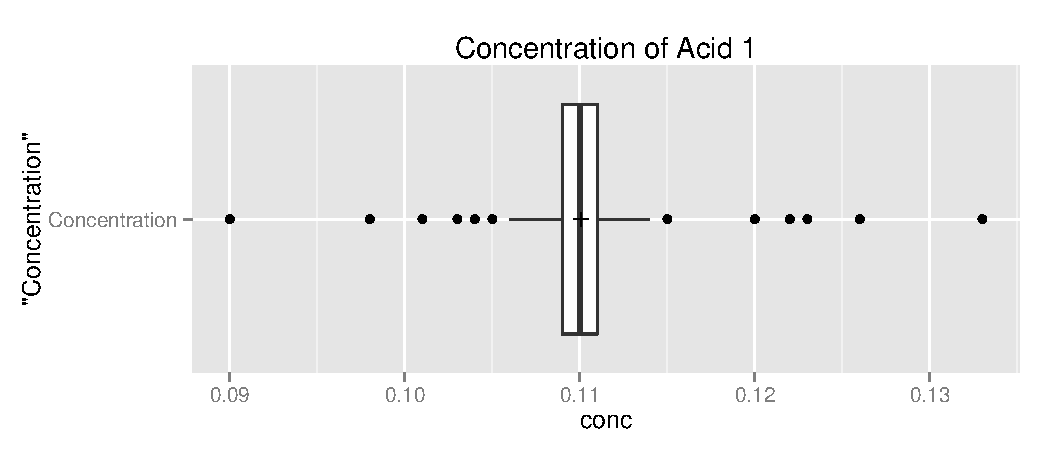
\includegraphics[width=\maxwidth]{figure/3a_box} 
\begin{kframe}\begin{alltt}
\hlstd{acid1.t} \hlkwb{<-} \hlkwd{t.test}\hlstd{(acid1}\hlopt{$}\hlstd{conc,} \hlkwc{mu} \hlstd{=} \hlnum{0.110}\hlstd{)}  \hlcom{# t-test summary}
\hlstd{acid1.t}
\end{alltt}
\begin{verbatim}
## 
## 	One Sample t-test
## 
## data:  acid1$conc
## t = 0.1581, df = 123, p-value = 0.8746
## alternative hypothesis: true mean is not equal to 0.11
## 95 percent confidence interval:
##  0.1093 0.1109
## sample estimates:
## mean of x 
##    0.1101
\end{verbatim}
\begin{alltt}
\hlstd{acid1.ybar} \hlkwb{<-} \hlkwd{mean}\hlstd{(acid1}\hlopt{$}\hlstd{conc)}  \hlcom{# mean of sample}
\hlstd{acid1.s} \hlkwb{<-} \hlkwd{sd}\hlstd{(acid1}\hlopt{$}\hlstd{conc)}       \hlcom{# standard deviation}
\hlstd{acid1.n} \hlkwb{<-} \hlkwd{length}\hlstd{(acid1}\hlopt{$}\hlstd{conc)}   \hlcom{# observations in sampe}
\hlstd{acid1.SEM} \hlkwb{<-} \hlstd{s}\hlopt{/}\hlkwd{sqrt}\hlstd{(acid1.n)}    \hlcom{# standard error of the mean}
\hlstd{acid1.df} \hlkwb{<-} \hlstd{acid1.n} \hlopt{-} \hlnum{1}         \hlcom{# degrees of freedom}
\hlstd{acid1.tcrit} \hlkwb{<-}\hlkwd{qt}\hlstd{(}\hlnum{.025}\hlstd{, acid1.df)}\hlcom{# t_crit}
\hlstd{acid1.M} \hlkwb{<-} \hlkwd{median}\hlstd{(acid1}\hlopt{$}\hlstd{conc)}   \hlcom{# median}
\hlstd{acid1.IQR} \hlkwb{<-} \hlkwd{IQR}\hlstd{(acid1}\hlopt{$}\hlstd{conc)}
\end{alltt}
\end{kframe}
\end{knitrout}

\begin{knitrout}
\definecolor{shadecolor}{rgb}{0.969, 0.969, 0.969}\color{fgcolor}\begin{kframe}
\begin{alltt}
\hlkwd{bs.one.samp.dist}\hlstd{(acid1}\hlopt{$}\hlstd{conc)}      \hlcom{# plot histogram and frequency density curve}
\end{alltt}
\end{kframe}
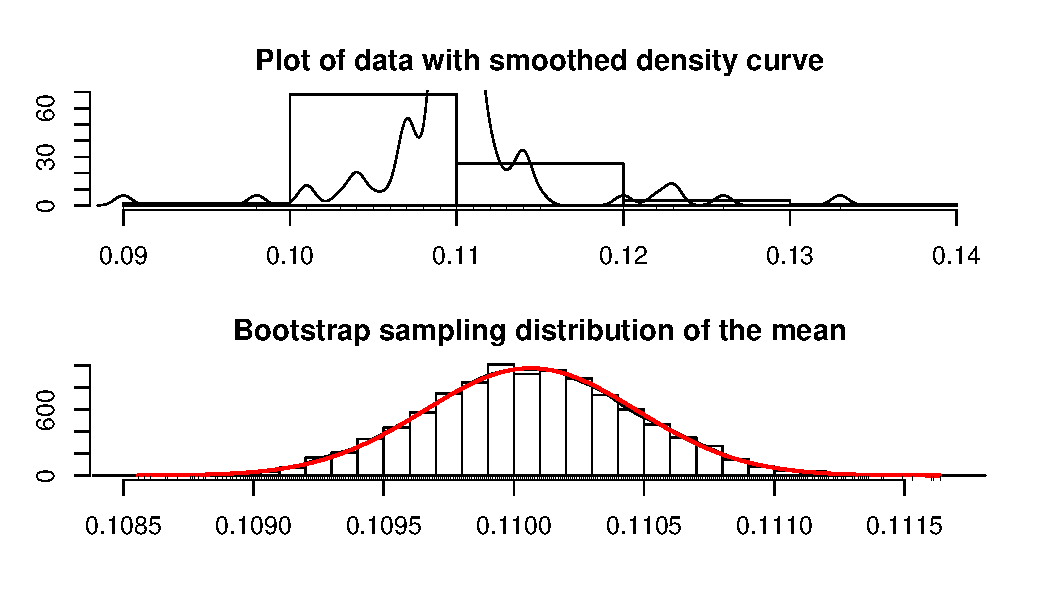
\includegraphics[width=\maxwidth]{figure/3a_hist} 

\end{knitrout}

\begin{itemize}
  \item \textbf{define the population parameter:} The population parameter is
  the mean measured acidity of the solution ($\mu = $ mean acidity of solution).

  \item \textbf{state the hypothesis:}  The hypothesis is that the students did
  not have a bias ($H_0: \mu = 0.110$ against $H_A: \mu \neq 0.110$).

  \item \textbf{state assumptions and how they will be assessed:}  The assumptions for
  this analysis are that the data are normally distributed.  Also, I will
  assume the entire population was sampled.

  \item
  Based on the histogram of the sample data, the data are unimodal, symmetric,
  and nearly normal.  Based on the bootstrap distribution, the sample data are
  normally distributed.  The boxplot of sample data shows outliers
  do exist, the tails are approximately equal, and the mean is essentially the meadian.

  The sample summaries are $n = 124, \bar{Y} = 0.110, s = 0.005 \text{ and }
  SE_{\bar{Y}} = 1.28$.  $\bar{Y} - M = 0.110 - 0.110 = 0$ is very small
  relative to the variability, which is consistent with the observed symmetry.

  \item
  I fail to reject $H_0$ in favor of $H_A$.  This test was performed at a 5\% level
  (i.e. $\alpha = 0.05$), and the p-value (0.8747) is $\ge \alpha$ and
  accordingly $t_s (0.1581) \le t_{crit}(1.979)$.  The data suggest that
  $\mu = 0.110$.  Additionally, I am 95\% confident that the population
  mean is $0.110 \pm 8e-4$, and the students were not biased for experiment 1.
\end{itemize}

\subsection{Acid 2}
\begin{knitrout}
\definecolor{shadecolor}{rgb}{0.969, 0.969, 0.969}\color{fgcolor}\begin{kframe}
\begin{alltt}
\hlcom{# boxplot of Unseeded acid1}
\hlstd{acid2.box} \hlkwb{<-} \hlkwd{ggplot}\hlstd{(acid2,} \hlkwd{aes}\hlstd{(}\hlkwc{x} \hlstd{=} \hlstr{"Concentration"}\hlstd{,} \hlkwc{y} \hlstd{= conc))} \hlcom{# boxplot of acid2}
\hlstd{acid2.box} \hlkwb{<-} \hlstd{acid2.box} \hlopt{+} \hlkwd{geom_boxplot}\hlstd{()}
\hlstd{acid2.box} \hlkwb{<-} \hlstd{acid2.box} \hlopt{+} \hlkwd{coord_flip}\hlstd{()}
\hlstd{acid2.box} \hlkwb{<-} \hlstd{acid2.box} \hlopt{+} \hlkwd{stat_summary}\hlstd{(}\hlkwc{fun.y} \hlstd{= mean,} \hlkwc{geom} \hlstd{=} \hlstr{"point"}\hlstd{,} \hlkwc{shape} \hlstd{=} \hlnum{3}\hlstd{,} \hlkwc{size} \hlstd{=} \hlnum{2}\hlstd{)}
\hlstd{acid2.box} \hlkwb{<-} \hlstd{acid2.box} \hlopt{+} \hlkwd{labs}\hlstd{(}\hlkwc{title} \hlstd{=} \hlstr{"Concentration of Acid 2"}\hlstd{)}
\hlstd{acid2.box}
\end{alltt}
\end{kframe}
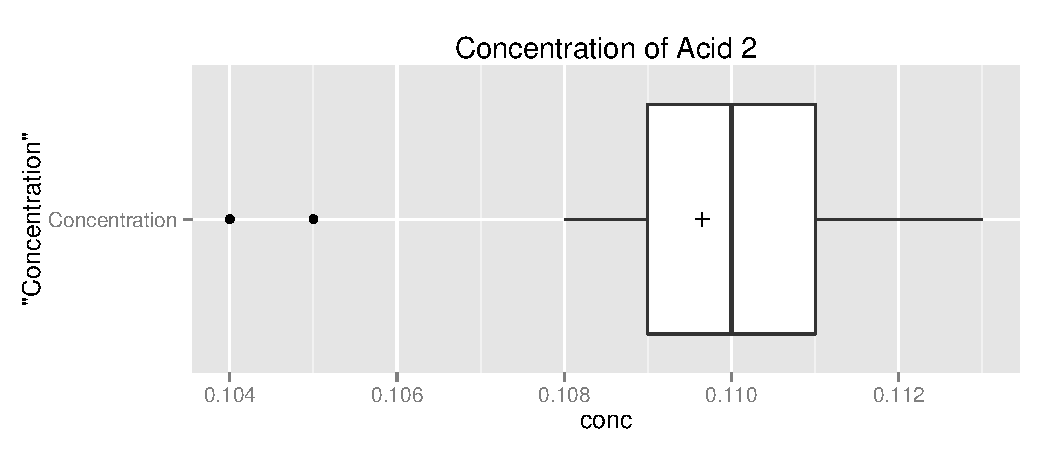
\includegraphics[width=\maxwidth]{figure/3b_box} 
\begin{kframe}\begin{alltt}
\hlstd{acid2.t} \hlkwb{<-} \hlkwd{t.test}\hlstd{(acid2}\hlopt{$}\hlstd{conc,} \hlkwc{mu} \hlstd{=} \hlnum{0.110}\hlstd{)}  \hlcom{# t-test summary}
\hlstd{acid2.t}
\end{alltt}
\begin{verbatim}
## 
## 	One Sample t-test
## 
## data:  acid2$conc
## t = -1.159, df = 36, p-value = 0.2541
## alternative hypothesis: true mean is not equal to 0.11
## 95 percent confidence interval:
##  0.1090 0.1103
## sample estimates:
## mean of x 
##    0.1096
\end{verbatim}
\begin{alltt}
\hlstd{acid2.ybar} \hlkwb{<-} \hlkwd{mean}\hlstd{(acid2}\hlopt{$}\hlstd{conc)}  \hlcom{# mean of sample}
\hlstd{acid2.s} \hlkwb{<-} \hlkwd{sd}\hlstd{(acid2}\hlopt{$}\hlstd{conc)}       \hlcom{# standard deviation}
\hlstd{acid2.n} \hlkwb{<-} \hlkwd{length}\hlstd{(acid2}\hlopt{$}\hlstd{conc)}   \hlcom{# observations in sampe}
\hlstd{acid2.SEM} \hlkwb{<-} \hlstd{s}\hlopt{/}\hlkwd{sqrt}\hlstd{(acid2.n)}    \hlcom{# standard error of the mean}
\hlstd{acid2.df} \hlkwb{<-} \hlstd{acid2.n} \hlopt{-} \hlnum{1}         \hlcom{# degrees of freedom}
\hlstd{acid2.tcrit} \hlkwb{<-}\hlkwd{qt}\hlstd{(}\hlnum{.025}\hlstd{, acid2.df)}\hlcom{# t_crit}
\hlstd{acid2.M} \hlkwb{<-} \hlkwd{median}\hlstd{(acid2}\hlopt{$}\hlstd{conc)}   \hlcom{# median}
\hlstd{acid2.IQR} \hlkwb{<-} \hlkwd{IQR}\hlstd{(acid2}\hlopt{$}\hlstd{conc)}
\end{alltt}
\end{kframe}
\end{knitrout}

\begin{knitrout}
\definecolor{shadecolor}{rgb}{0.969, 0.969, 0.969}\color{fgcolor}\begin{kframe}
\begin{alltt}
\hlkwd{bs.one.samp.dist}\hlstd{(acid2}\hlopt{$}\hlstd{conc)}      \hlcom{# plot histogram and frequency density curve}
\end{alltt}
\end{kframe}
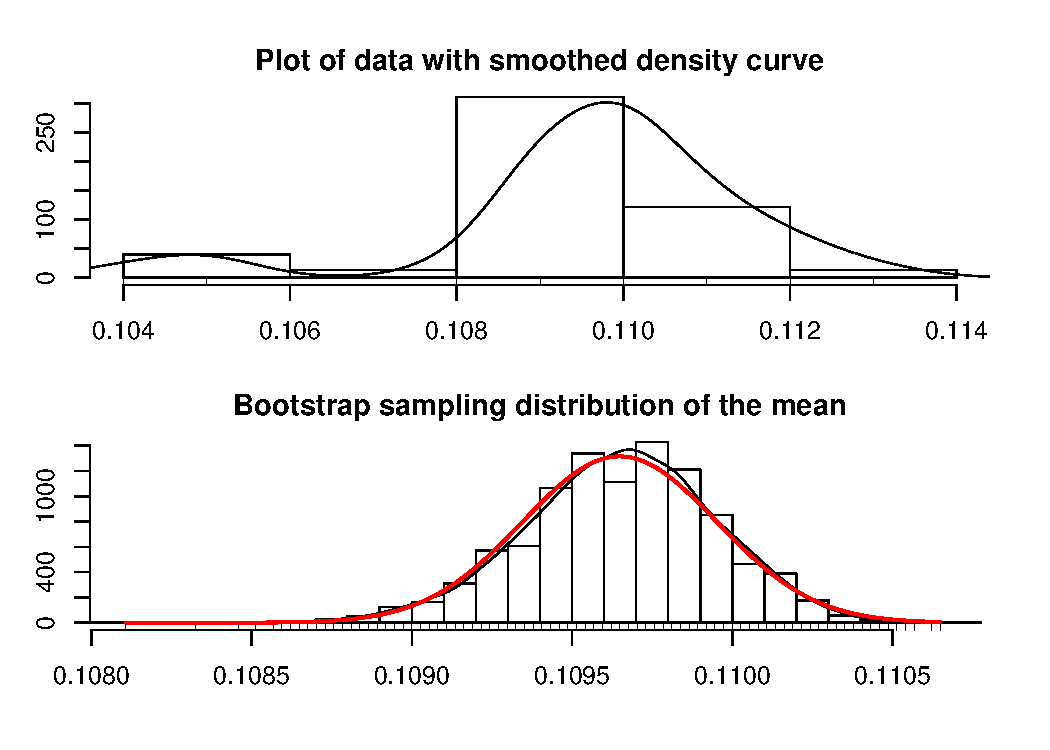
\includegraphics[width=\maxwidth]{figure/3b_hist} 

\end{knitrout}

\begin{itemize}
  \item \textbf{define the population parameter:} The population parameter is
  the mean measured acidity of the solution ($\mu = $ mean acidity of solution).

  \item \textbf{state the hypothesis:}  The hypothesis is that the students did
  not have a bias ($H_0: \mu = 0.110$ against $H_A: \mu \neq 0.110$).

  \item \textbf{state assumptions and how they will be assessed:}  The assumptions for
  this analysis are that the data are normally distributed, and that the entire
  population was sampled.

  \item
  Based on the histogram of the sample data, the data are unimodal, skewed left,
  and not normal.  Based on the bootstrap distribution, the sample are
  normally distributed.  The boxplot of sample data shows that outliers
  do exist, the tails are not equal, and the mean noticeably different than
  the meadian.

  The sample summaries are $n = 37, \bar{Y} = 0.1096, s = 0.002 \text{ and }
  SE_{\bar{Y}} = 2.34$.  $\bar{Y} - M = 0.1096 - 0.110 = -4e-4$, which is
  orders of magnitude smaller than the IQR.

  \item
  I fail to reject $H_0$ in favor of $H_A$.  This test was performed at a 5\% level
  (i.e. $\alpha = 0.05$), and the p-value (0.8747) is $\ge \alpha$ and
  accordingly $t_s (0.1581) \le t_{crit}(1.979)$. In a valid t-test, this results
  would indicate the null hypothesis should be rejected, but because the
  normality assumption was not met, I choose to accept the null hypothesis.

  $\mu = 0.110$.  Additionally, I am 95\% confident that the population
  mean is $0.1096 \pm 0.00065$, and the students were not biased for experiment 2.
\end{itemize}

\end{document}
